%=========================================================

% Here you can choose if compile with or without solutions.
% However, this definition is ignored if you use any
% command from the `Makefile`.
\providecommand{\withSol}{\iftrue}

%=========================================================

\documentclass
[twoside,english,colorbacktitle,accentcolor=tud9c]
{tudexercise}

\usepackage[T1]{fontenc}
\usepackage[latin9]{inputenc}
\usepackage{amstext}
\usepackage{amsmath}
\usepackage{graphicx}
\usepackage{setspace}
\usepackage{multicol}
\usepackage{mathtools}
\usepackage{dsfont}
\usepackage{units}
\usepackage{subfigure}
\usepackage{color}
\usepackage{booktabs}
\usepackage{fancyref}
\usepackage{parskip}
\usepackage[ngerman,english]{babel}

%=========================================================

\def\homework{3}
\def\homeworkVer{1}
\def\homeworkSolVer{1}

%=========================================================

\ifcsname withSol\endcsname\else
  \expandafter\let\csname withSol\expandafter\endcsname
                  \csname iffalse\endcsname
\fi

\withSol
	\usepackage[solutions]{iasHomework}
\else
	\usepackage{iasHomework}
\fi

%=========================================================

\hwtitle{Machine Learning}
{Summer Semester 2016}
{Prof. Dr. J. Peters, F. Veiga, S. Parisi}

\begin{document}

%=========================================================

\maketitle

\begin{examheader}
	\textmb{Machine Learning - Homework \arabic{section}}
	\examheaderdefault 
\end{examheader} 

\deadline{Wednesday, 22 June 2016 (before the lecture)}

%=========================================================

\newif\ifvimbug
\vimbugfalse

\ifvimbug
\begin{document}
\fi

\exercise{Linear Regression}

In this exercise, you will use the dataset \texttt{linRegData.txt}, containing $150$ points in the format \texttt{<input variable, output variable>}. The input is generated by a sinusoid function, while the output is the joint trajectory of a compliant robotic arm. 
The first $N=20$ data points are the training set and the remainder are the testing set.

\begin{questions}

%----------------------------------------------

\begin{question}{Polynomial Features}{10}
Write the equation of the model and fit it with polynomial features. Using the Root Mean Square Error (RMSE) as a metric for the evaluation, select the complexity of the model (up to a 21st degree polynomial) by evaluating its performance the on testing data. Which is the best RMSE you achieve and what is the model complexity? Does it change if we evaluate our model on the training data? Comment your findings and plot the RMSE for each case (use two lines, one for evaluation on training data, one for evaluation on testing data).
For the estimation of the optimal parameters use a Ridge coefficient of $\lambda=10^{-6}$.

Using what you think is the best learned model from the previous point, show in a single plot the ground truth (full dataset) and the model prediction over it.
Attach snippets of your code showing how you generate polynomial features and how you fit the model.


\begin{answer}
In order to create polynomial features of degree n, the function exprepeat is used. It calculates the matrix $X$, based on the given vector
$x = (\begin{matrix}
x_k\\
\vdots\\
x_1\\
x_0\\
\end{matrix})$ as 
$X = (
\begin{matrix*}
	x_0^n & x_1^n & \hdots & x_k^n\\
	\vdots & \ddots & \hdots & \vdots\\
	x_0 & x_1 & \hdots & x_k\\
	1 & 1 & \hdots & 1
\end{matrix*}
)$
\lstinputlisting[language=Python, firstline= 5, lastline = 15]{../Code/31a.py}

The polynomial features are then used in polyregress to calculate the coefficients of the polynomial of degree n, according to the formula in the lecture: $w=(XX^T)^{-1}Xy$

\lstinputlisting[language=Python, firstline= 17, lastline = 24]{../Code/31a.py}

Based on these results, the polynomial is first evaluated at all available data points, using $y_{fit} = w^TX$. The RMSE is than calculated as $\sqrt{\sum_{n=0}^{N-1}\frac{ (y_{fit,n}-y_n)^2}{N}}$, where $N$ is the number of samples in the dataset. This is done separately for the test and training set.

\lstinputlisting[language=Python, firstline= 25, lastline = 28]{../Code/31a.py}

The resulting RMSE for train and test data are plotted in the follwing figure.

\centering 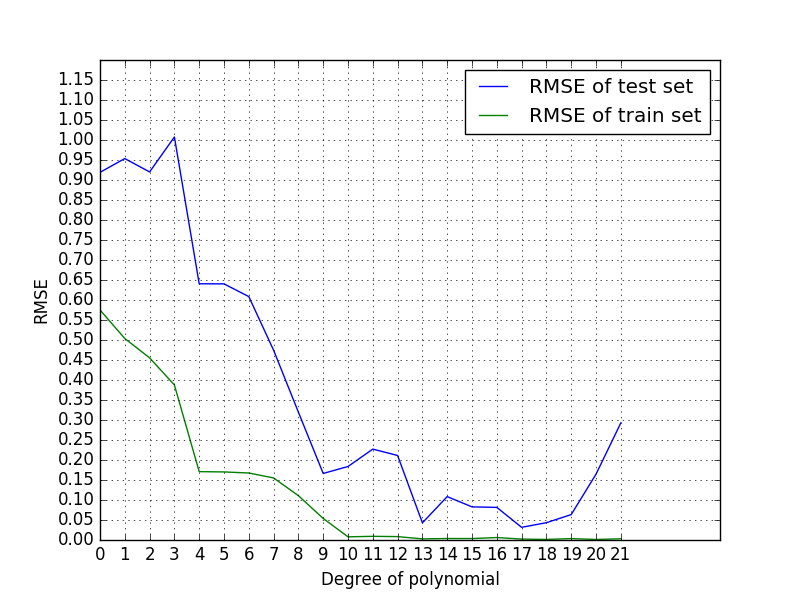
\includegraphics[width=0.7\linewidth]{img/31a}

As the plot shows, the RMSE of the training set is always lower than the one of the test set. This is not surprising, since the regression is trying to minimize the error for the training set. The lowest RMSE for the test set is achieved by using a polynomial of degree 17. This polynomial is shown in the following figure.

\centering 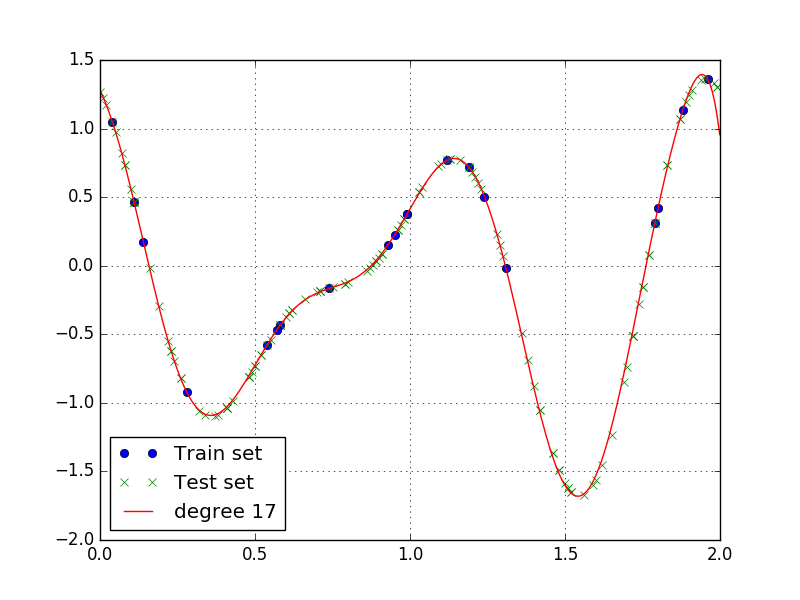
\includegraphics[width=0.7\linewidth]{img/31a2}

	
\end{answer}

\end{question}

%----------------------------------------------

\begin{question}{Gaussian Features}{4}
Now use Gaussian features. Each feature is a Gaussian distribution were the means are distributed linearly in $x \in[0,2]$ and the variance is set to $\sigma^2=0.02$. The features have to be normalized, i.e., they have to sum to one at every state. Using $N=20$ features generate a plot with the activation of each feature over time (i.e., plot the matrix $\Phi$). Attach a snippet of your code showing how to compute Gaussian features.

\begin{answer}
\centering 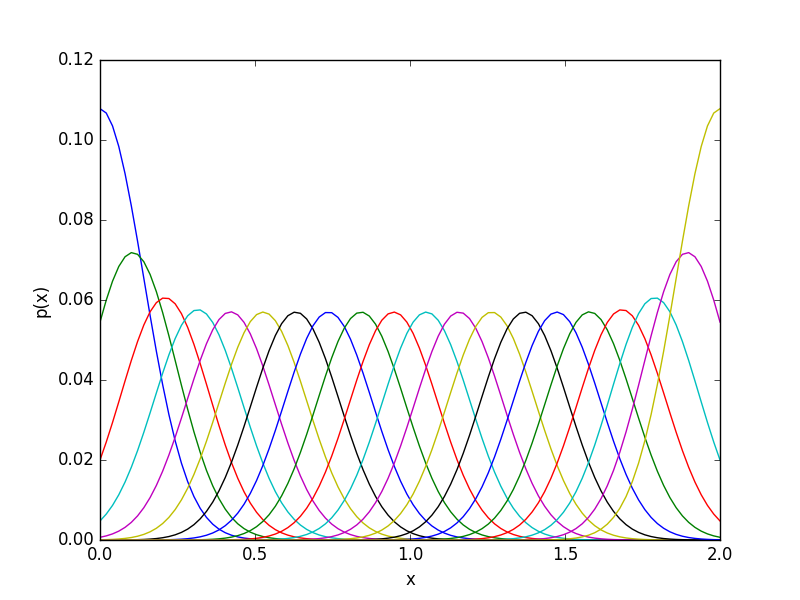
\includegraphics[width=1.0\linewidth]{img/31b}\label{fig:gaussians}

\lstinputlisting[language=Python, firstline = 11]{../Code/31b.py}

\end{answer}

\end{question}

%----------------------------------------------

\begin{question}{Gaussian Features, Continued}{6}
Repeat the process of fitting the model using the Gaussian features from the previous question. Compare the RMSE on the testing data using $15 \ldots 40$ basis functions and plot the RMSE. Which number of basis functions has the best performance and what is the best RMSE? Use a Ridge coefficient of $\lambda=10^{-6}$.

\begin{answer}\end{answer}
The best RMSE is $0.015431$ using 29 basis functions. \\
\centering 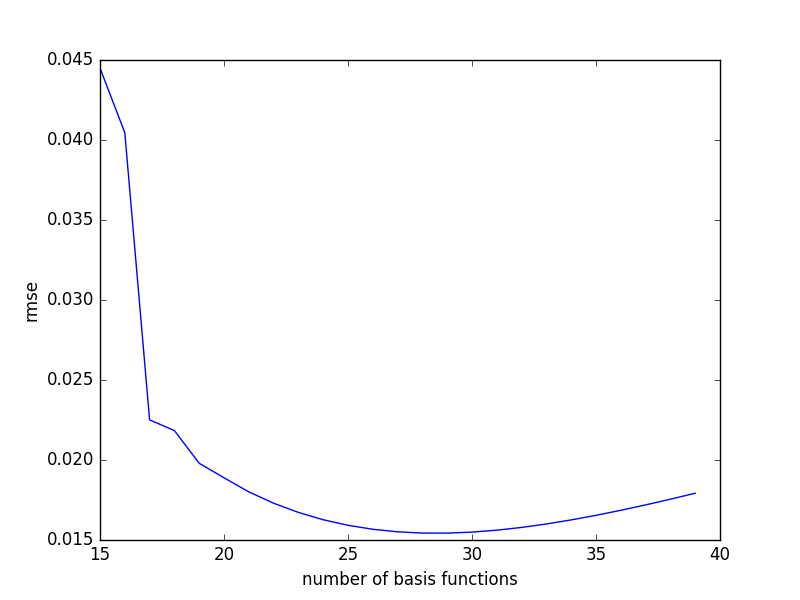
\includegraphics[width=1.0\linewidth]{img/31c_rmse}\label{fig:gaussians_rmse}

\end{question}

%----------------------------------------------

\begin{question}{Bayesian Linear Regression}{10}
Using Bayesian linear regression and polynomial features of 12th degree, plot the mean and the standard deviation of the predictive distribution for each case, using the first $N={10, 12, 16, 20, 50, 150}$ data points.
Discuss how the model uncertainty change with the amount of data points and the problem of overfitting with Bayesian linear regression. Use a prior $\sigma^2=0.0025$.

\begin{answer}
The uncertainty is getting lower the more data points we use for learning. This can be seen especially in the plot for $N=10$, where the area between data points is very uncertain, due to the lack of available information. However, the more points we have the less uncertain we are about our prediction. Regarding overfitting the bayesian linear regression performs better than MLE, because instead of optimizing we are integrating over all possible choices.

\centering 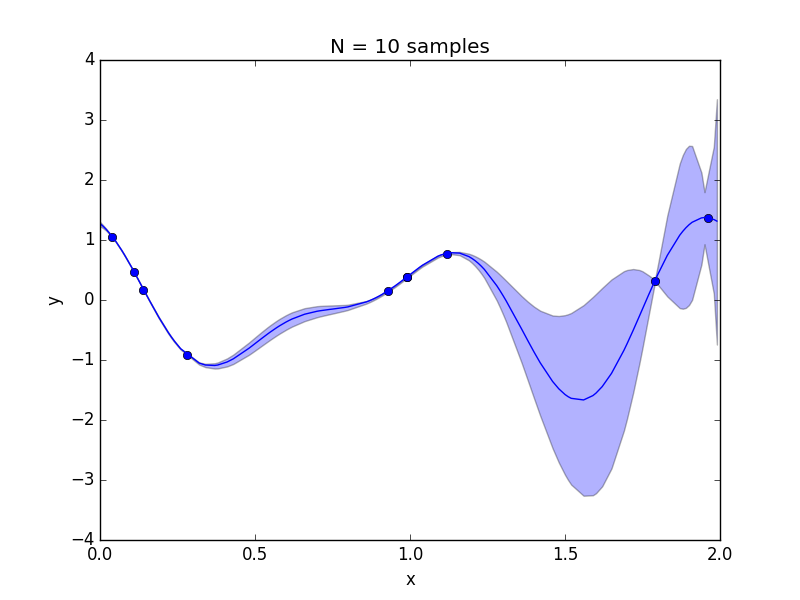
\includegraphics[width=1.0\linewidth]{img/31d_10} \\
\centering 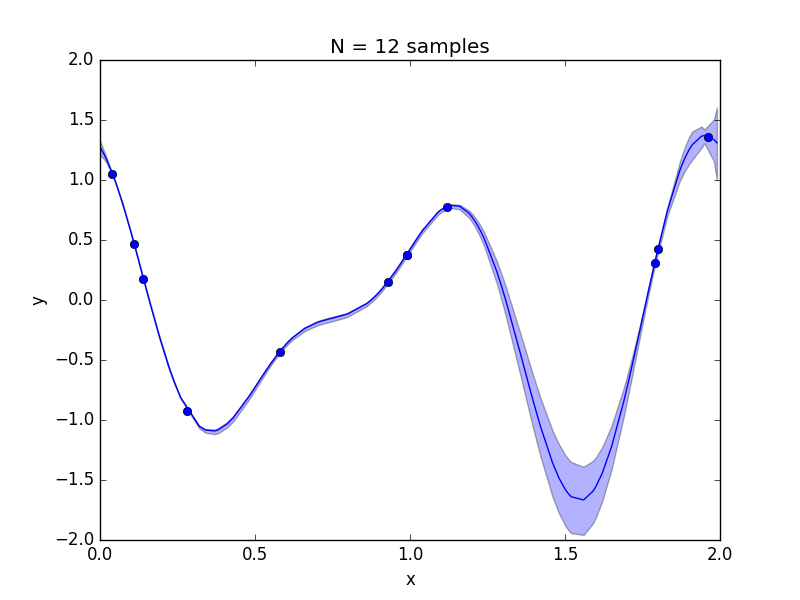
\includegraphics[width=1.0\linewidth]{img/31d_12} \\
\centering 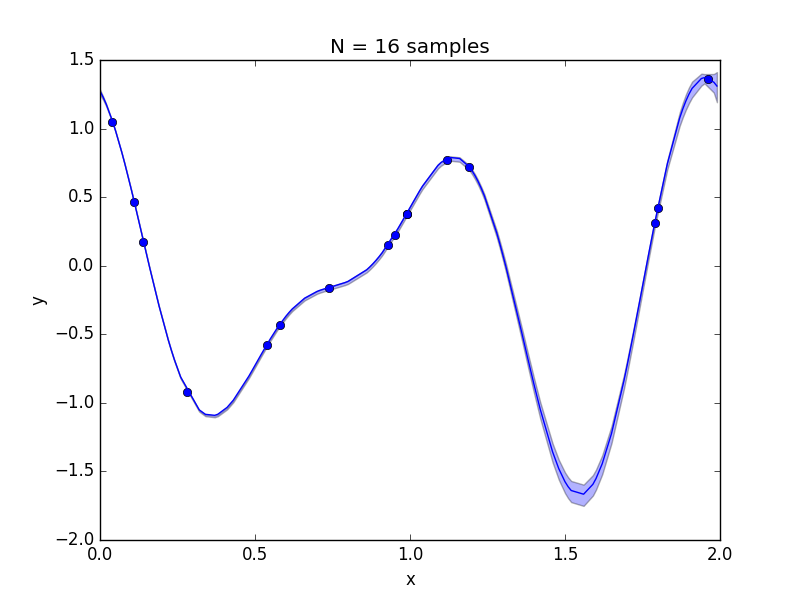
\includegraphics[width=1.0\linewidth]{img/31d_16} \\
\centering 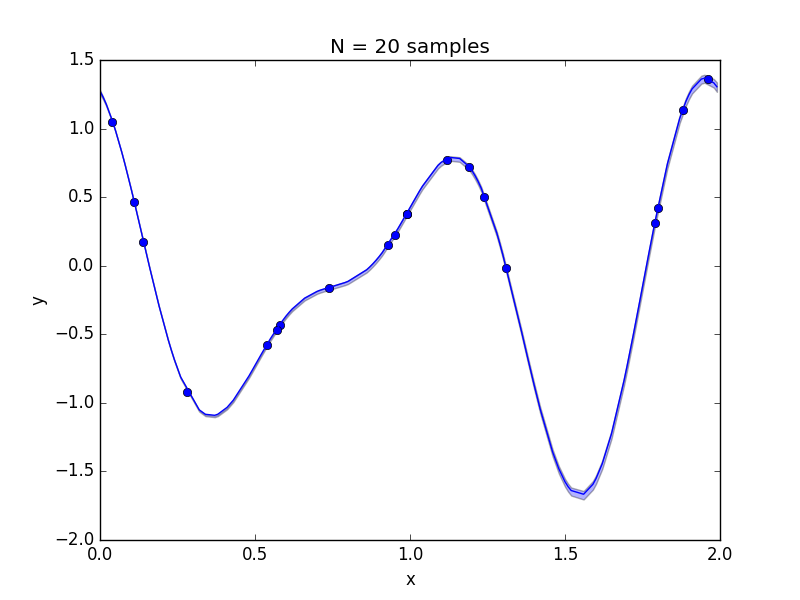
\includegraphics[width=1.0\linewidth]{img/31d_20} \\
\centering 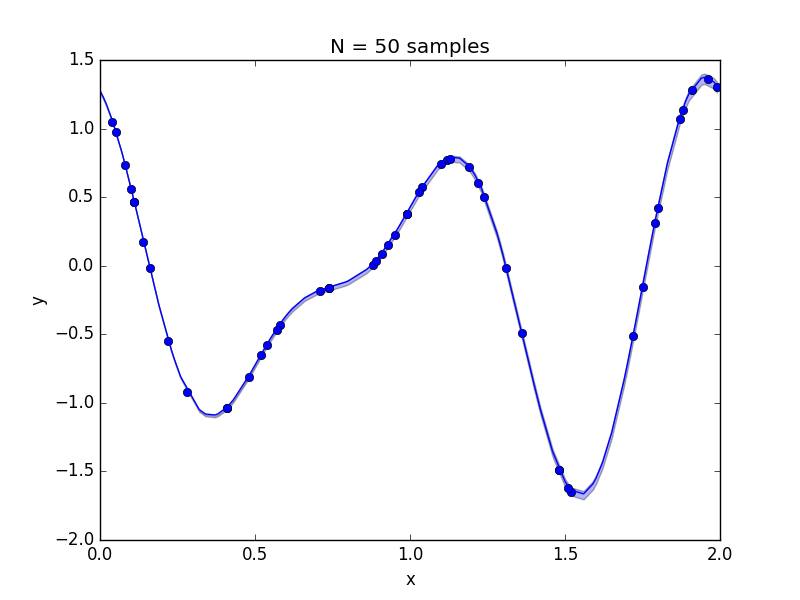
\includegraphics[width=1.0\linewidth]{img/31d_50} \\
\centering 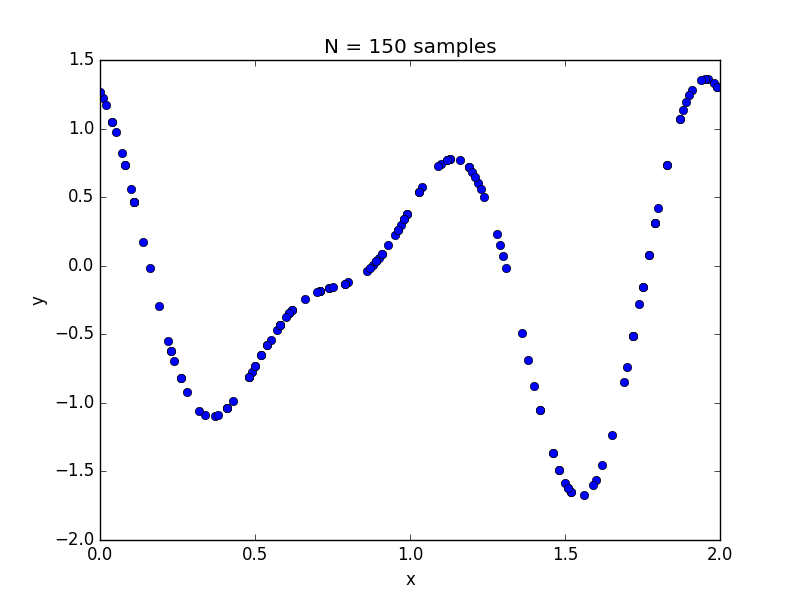
\includegraphics[width=1.0\linewidth]{img/31d_150}


\end{answer}
\end{question}

%----------------------------------------------

\begin{question}{Bayesian Linear Regression, Continued}{5}
How can we further reduce the uncertainty? Is it always a good practice?

\begin{answer}\end{answer}
\end{question}

%----------------------------------------------

\begin{question}[bonus]{Cross Validation}{5}
So far, we have split our dataset in two sets: training data and testing data. Cross-validation is a more sophisticated approach for model selection. Discuss it and its variants, pointing out their pro and cons.
\end{question}

\begin{answer}
When the original dataset is simply split into training- and test-set has the drawback, that evaluations based on this approach tend to reflect the particular characteristics of the splits. One may use statistical sampling to get better results. There are two cross-validation strategies:\\
\textbf{k-fold cross-validation}: The data is divided into $k$ different chunks (of same size), which are each used once as the learning-set in $k$ runs. Validation takes place on the respective training-sets in each run.\\
This method can be improved by choosing the $k$ chunks in a way, that data-points are similarly distributed in all chunks. This is called \textbf{stratified k-fold cross-validation} and reduces the predictions variance. \\
\textbf{Leave-one-out validation}: The data is divided in $N$ chunks of data, one for each data-point. This results in $N$ runs, which can lead to severe runtimes. In addition a stratified version is not possible. Furthermore there are extreme cases, in which the leave-one-out validation can give faulty results.
\end{answer}

\end{questions}


\newif\ifvimbug
\vimbugfalse

\ifvimbug
\begin{document}
\fi

\exercise{Linear Classification}

In this exercise, you will use the dataset \texttt{ldaData.txt}, containing $150$ feature points $\vec x$. The first 50 points belong to class $C_1$, the second 50 to class $C_2$, the last 50 to class $C_3$.


\begin{questions}
%----------------------------------------------

\begin{question}{Discriminative and Generative Models}{4}
Explain the difference between discriminative and generative models and give an example for each case.
Which model category is generally easier to learn and why?
 
\begin{answer}
Discriminative models don't directly calculate an underlying distribution. Instead, they use discriminant functions and the resulting class depends on the result of this function on a given point $x$. Discriminative models are easier to learn than generative models, because they depend less on details of a given distribution.

Generative models calculate the distribution of each class. This makes them more general, but they require more calculation steps.
	
\end{answer}

\end{question}

%----------------------------------------------

\begin{question}{Linear Discriminant Analysis}{12}
Use Linear Discriminant Analysis to classify the points in the dataset. Attach two plots with the data points using using a different color for each class: one plot with the original dataset, one with the samples classified according to your LDA classifier. Attach a snippet of your code and discuss the results. How many samples are misclassified? (You are allowed to use built-in functions for computing the mean and the covariance.)

\begin{answer}\end{answer}
\end{question}

%----------------------------------------------

\end{questions}


\newif\ifvimbug
\vimbugfalse

\ifvimbug
\begin{document}
\fi

\exercise{Principle Component Analysis}
In this exercise you will use the \texttt{Iris.txt} dataset. It contains data from three kind of Iris flowers (`Setosa', `Versicolour' and `Virginica') with 4 attributes: sepal length, sepal width, petal length, and petal width. Each row contains a sample while the last attribute is the label. A label of $0$ means that the sample comes from a `Setosa' plant, $1$ from a `Versicolour', and $2$ from `Virginica'.
(You are allowed to use built-in functions for computing the mean, the covariance, eigevalues and eigenvectors.)

\begin{questions}

%----------------------------------------------

\begin{question}{Data Normalization}{4}
Normalizing the data is a common practice in machine learning. Normalize the provided dataset such as it has zero mean and unit variance per dimension. Why is normalizing important?
Attach a snippet of your code. 

\begin{answer}
Subtracting the mean of the dataset is important, because otherwise the results of the Principal component analysis would be meaningless. Normalizing for unit variance prevents variables with a large variance to influence the PCA too significantly.

The normalization is done by the following function:
\lstinputlisting[language=Python, firstline=11, lastline = 21]{../Code/33a.py}
	
\end{answer}

\end{question}

%----------------------------------------------

\begin{question}{Principle Component Analysis}{8}
Apply PCA on your normalized dataset and generate a table showing the proportion (percentage) of cumulative variance explained. 
How many components do you need in order to explain at least $95\%$ of the dataset variance? 
Attach a snippet of your code.

\begin{answer}
The Principal Component Analysis of a normalized dataset X can be computed using the following snippet:

\lstinputlisting[language=Python, firstline=25, lastline=28]{../Code/33a.py}



The cumulative explained variance of these Eigenvalues is 
\[
\begin{array}{c|c|c|c}
\lambda_1& \lambda_2 & \lambda_3 & \lambda_4 \\ \hline
0.72770452 & 0.95800975 & 0.99484807 & 1.
\end{array} 
\]

Therefore, in order to explain more than 95\% variance, 2 Eigenvectors are needed.
	
\end{answer}

\end{question}

%----------------------------------------------

\begin{question}{Low Dimensional Space}{6}
Using as many components as needed to explain $95\%$ of the dataset variance, generate a scatter plot of the lower-dimensional projection of the data. Use different colors or symbols for data points from different classes. 
What do you observe? Attach a snippet of your code.

\begin{answer}
The first step is to project the data. This is done by a simple dot-multiplication. In the snippet, the dataset is transposed because of the order of the data in the given file. The result is transposed to restore that order:
\lstinputlisting[language=Python, firstline=64, lastline=65]{../Code/33a.py}


The data is plotted using the following snippet, where C0, C1 and C2 indicate the samples that belong to the corresponding class:
\lstinputlisting[language=Python, firstline=67, lastline=74]{../Code/33a.py}

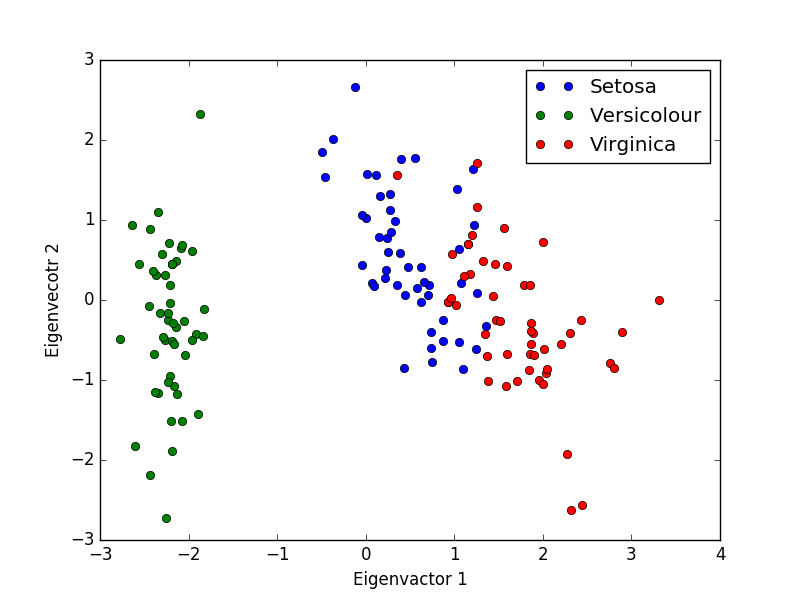
\includegraphics[width=1.0\linewidth]{./img/33c.png}

From this perspective, the plant Versicolour is easily separable from the other two plants. Setosa and Virginica are also separated, but they overlap.

\end{answer}

\end{question}

%----------------------------------------------

\begin{question}{Projection to the Original Space}{6}
Reconstruct the original dataset by using different number of principle components. Using the normalized root mean square error (NRMSE) as a metric, create a table with the error per input versus the amount of principle components used (i.e., with five columns: first for the number of components, remainder for the input NRMSE).
Attach a snippet of your code.
(Remember that in the first step you normalized the data.)


\begin{answer}


\[\begin{array}{lcccc}
	Components & 1 & 2 & 3 & 4 \\ 
	NRMSE & a & b & c & d
\end{array} 
\]
	
\end{answer}
\end{question}

\begin{question}[bonus]{Kernel PCA}{15}
Throughout this class we have seen that PCA is an easy and efficient way to reduce the dimensionality of some data. However, it is able to detect only linearly dependences among data points. A more sophisticated extension to PCA, \emph{Kernel PCA}, is able to overcome this limitation. 
This question asks you to deepen this topic by conducting some research by yourself: explain what Kernel PCA is, how it works and what are its main limitations. Be as much as concise (but clear) as possible.

\begin{answer}
The PCA decorrelates the features given in a dataset by diagonalizing the covariance matrix, given by 
\[S = \frac{1}{N} \sum_{n=1}^{N}x_n x_n^T\]
Unfortunately, this only works well, if the relation between the feature is linear.

To circumvent this problem, a transformation $\Phi (x)$ can be used to project the samples into a feature space. In an ideal feature space, the relations between two different features are only linear. Consider an example, where two features, $x_{(1)}$ and $x_{(2)}$ have a quadratic relationship: $x_{(2)} = 5 \cdot x_{(1)}^2$. A transformation $\Phi(x) = (\begin{matrix}
x_{(1)}^2\\
x_{(2)}
\end{matrix}) $ would make this relationship linear and therefore PCA applicable.

This means, that in Kernel PCA, the covariance matrix of the feature space 
\[S'=\frac{1}{N} \sum_{n=1}^{N} \Phi(x_n) \Phi(x_n)^T\]
is diagonalized by solving its eigenvector equation \[S'v_i = \lambda_i v_i\]

However, transforming every sample into the feature space by applying $\Phi(x)$ is a very computation intensive operation. Therefore, the goal is to solve this eigenvector problem without having to work in the feature space.  
 
\end{answer}

\end{question}

\end{questions}


%=========================================================

\end{document}

